% Options for packages loaded elsewhere
\PassOptionsToPackage{unicode}{hyperref}
\PassOptionsToPackage{hyphens}{url}
%
\documentclass[
]{article}
\usepackage{amsmath,amssymb}
\usepackage{lmodern}
\usepackage{ifxetex,ifluatex}
\ifnum 0\ifxetex 1\fi\ifluatex 1\fi=0 % if pdftex
  \usepackage[T1]{fontenc}
  \usepackage[utf8]{inputenc}
  \usepackage{textcomp} % provide euro and other symbols
\else % if luatex or xetex
  \usepackage{unicode-math}
  \defaultfontfeatures{Scale=MatchLowercase}
  \defaultfontfeatures[\rmfamily]{Ligatures=TeX,Scale=1}
\fi
% Use upquote if available, for straight quotes in verbatim environments
\IfFileExists{upquote.sty}{\usepackage{upquote}}{}
\IfFileExists{microtype.sty}{% use microtype if available
  \usepackage[]{microtype}
  \UseMicrotypeSet[protrusion]{basicmath} % disable protrusion for tt fonts
}{}
\makeatletter
\@ifundefined{KOMAClassName}{% if non-KOMA class
  \IfFileExists{parskip.sty}{%
    \usepackage{parskip}
  }{% else
    \setlength{\parindent}{0pt}
    \setlength{\parskip}{6pt plus 2pt minus 1pt}}
}{% if KOMA class
  \KOMAoptions{parskip=half}}
\makeatother
\usepackage{xcolor}
\IfFileExists{xurl.sty}{\usepackage{xurl}}{} % add URL line breaks if available
\IfFileExists{bookmark.sty}{\usepackage{bookmark}}{\usepackage{hyperref}}
\hypersetup{
  pdftitle={PS6 homework},
  pdfauthor={Ahmed},
  hidelinks,
  pdfcreator={LaTeX via pandoc}}
\urlstyle{same} % disable monospaced font for URLs
\usepackage[margin=1in]{geometry}
\usepackage{graphicx}
\makeatletter
\def\maxwidth{\ifdim\Gin@nat@width>\linewidth\linewidth\else\Gin@nat@width\fi}
\def\maxheight{\ifdim\Gin@nat@height>\textheight\textheight\else\Gin@nat@height\fi}
\makeatother
% Scale images if necessary, so that they will not overflow the page
% margins by default, and it is still possible to overwrite the defaults
% using explicit options in \includegraphics[width, height, ...]{}
\setkeys{Gin}{width=\maxwidth,height=\maxheight,keepaspectratio}
% Set default figure placement to htbp
\makeatletter
\def\fps@figure{htbp}
\makeatother
\setlength{\emergencystretch}{3em} % prevent overfull lines
\providecommand{\tightlist}{%
  \setlength{\itemsep}{0pt}\setlength{\parskip}{0pt}}
\setcounter{secnumdepth}{-\maxdimen} % remove section numbering
\usepackage{booktabs}
\usepackage{longtable}
\usepackage{array}
\usepackage{multirow}
\usepackage{wrapfig}
\usepackage{float}
\usepackage{colortbl}
\usepackage{pdflscape}
\usepackage{tabu}
\usepackage{threeparttable}
\usepackage{threeparttablex}
\usepackage[normalem]{ulem}
\usepackage{makecell}
\usepackage{xcolor}
\ifluatex
  \usepackage{selnolig}  % disable illegal ligatures
\fi

\title{PS6 homework}
\author{Ahmed}
\date{03/22/2022}

\begin{document}
\maketitle

\hypertarget{cleaning-process}{%
\section{Cleaning process}\label{cleaning-process}}

\begin{tabular}{r|l|l|l|l|l|r}
\hline
DIVISION & STATE & COUNTY & STNAME & CTYNAME & CENSUS2010POP & ESTIMATESBASE2010\\
\hline
6 & 01 & 000 & Alabama & Alabama & 4779736 & 4780118\\
\hline
6 & 01 & 001 & Alabama & Autauga County & 54571 & 54582\\
\hline
6 & 01 & 003 & Alabama & Baldwin County & 182265 & 182263\\
\hline
6 & 01 & 005 & Alabama & Barbour County & 27457 & 27454\\
\hline
6 & 01 & 007 & Alabama & Bibb County & 22915 & 22904\\
\hline
6 & 01 & 009 & Alabama & Blount County & 57322 & 57322\\
\hline
\end{tabular}

The raw data from census comes in a wide format where years are attached
to the variable names (see the sample of raw data above). The first step
is to first gather the 180 columns using ``gather'' function in R. Next,
we create a year variable by parsing or extracting the year from the
string categories. We then omit the years in the category variable to
end up with unique list of variables. We can keep our data in the long
format or spread it again using ``spread'' function; I actually prefer
the latter format as it makes it easy to see and sort variables in R
studio. The cleaned data looks as follow:

\begin{tabular}{r|l|l|l|r|r|r|r}
\hline
year & county\_fips & STNAME & CTYNAME & POPESTIMATE & BIRTHS & RBIRTH & DEATHS\\
\hline
2010 & 01001 & Alabama & Autauga County & 54761 & 151 & NA & 157\\
\hline
2010 & 01003 & Alabama & Baldwin County & 183121 & 514 & NA & 534\\
\hline
2010 & 01005 & Alabama & Barbour County & 27325 & 70 & NA & 131\\
\hline
2010 & 01007 & Alabama & Bibb County & 22858 & 44 & NA & 32\\
\hline
2010 & 01009 & Alabama & Blount County & 57372 & 181 & NA & 132\\
\hline
2010 & 01011 & Alabama & Bullock County & 10876 & 37 & NA & 53\\
\hline
\end{tabular}

\hypertarget{net-migration}{%
\section{Net migration}\label{net-migration}}

While I cleaned this data primarily to merge it with my project data for
college enrollment and use only population and migration as controls, I
think it's interesting to visualize the net migration and see which
destinations, counties and states, attract more migration. Choropleth
map can be of a good use for this purpose. Thus, I used
\href{https://github.com/UrbanInstitute/urbnmapr}{``urbnmapr''} along
with ``ggplot''.

\hypertarget{visuals}{%
\subsection{Visuals}\label{visuals}}

\includegraphics{PS6_ElFatmaoui_files/figure-latex/unnamed-chunk-3-1.pdf}

\includegraphics{PS6_ElFatmaoui_files/figure-latex/unnamed-chunk-4-1.pdf}

The maps show the net migration per county and state in 2020. Florida,
Texas and probably even Arizona seem to have higher net migration
compared to any other states. The county map doesn't clearly show which
counties in these three states have higher migration. We can though see
that Maricopa county in Arizona, and Collin and Harris counties in Texas
are the most attractive migration destination.

Let's now closely look at which counties are driving these states high
migration.

\includegraphics{PS6_ElFatmaoui_files/figure-latex/unnamed-chunk-5-1.pdf}

The above plot looks too busy especially for Florida, so let's focus on
the upper and lower migration counties.

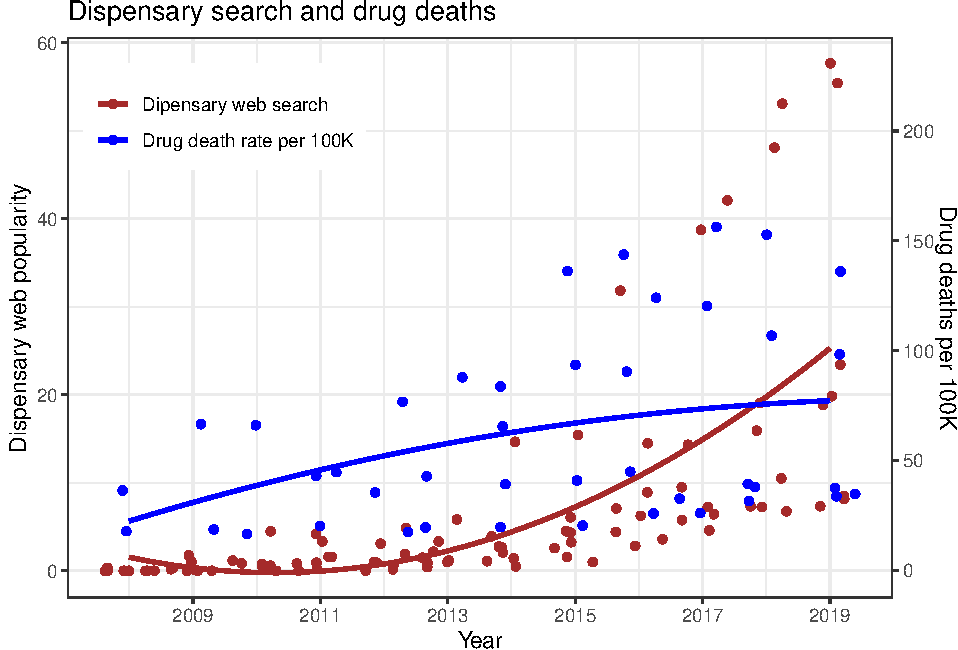
\includegraphics{PS6_ElFatmaoui_files/figure-latex/unnamed-chunk-6-1.pdf}
\includegraphics{PS6_ElFatmaoui_files/figure-latex/unnamed-chunk-6-2.pdf}

Arizona seem to have fewer counties with negative net migration. Miami
Dade and Dallas counties have gradually net negative migration
throughout the period. Harris county seem to have ups and downs in net
migration.

Future research ideas may entail learning about factors that drive
higher net migration in the discussed states. Some of the reasons are
probably already obvious, high prices and unemployment rate.

\end{document}
